\chapter{Related Work
    \pgsize{15 p.}
}
\label{chap:relatedwork}

\mnote{Related work on goal and methodology}
Collaboration is a key factor in software engineering processes and especially \gls{MDSD}, but also represents a key challenge, in particular due to the necessity of consistency preservation~\cite{franzago2018mdseChallenges-TSE}.
This thesis contributes to the goal of preserving consistency of different engineering artifacts or models and especially uses and extends the methodology of model transformations to achieve that goal.
We relate our research to existing work separated into two categories given by the general goal of consistency preservation, which primarily comprises different approaches to solve the underlying problem but with potentially different methodology, and the methodology of using transformations for consistency preservation and specific topics regarding transformations, their properties and their composition.

\begin{figure}
    \centering
    \begin{tikzpicture}[every node/.append style={font=\footnotesize}]

\draw[fill=darkred!10] (0.8em,0.5em) ellipse (3em and 3em);

\draw[darkgreen, thick] (0,0) ellipse (15em and 15em);
\node[darkgreen, anchor=north, align=center, font=\footnotesize\bfseries] at (0, 14em) {\emph{Goal:}\\ Consistency and its Preservation};
\draw[darkgreen, thick] (3em,-0.25em) ellipse (11.5em and 11.5em);
\node[darkgreen, anchor=north, align=center, font=\footnotesize\bfseries] at (3em, 10.25em) {\emph{Methodology:}\\ Consistency by Transformation};
\draw (-6.5em,4.5em) ellipse (7.5em and 3.5em);
\node[anchor=west, align=center] at (-12.5em, 5em) {View-Update\\ Problem};
\draw (-7em,-1em) ellipse (7.5em and 3.5em);
\node[anchor=west, align=center] at (-14em, -1em) {Traceability /\\ Model Merging};
\draw (-4em,-7em) ellipse (5.5em and 7em);
\node[anchor=south, align=center] at (-4em, -13.5em) {Constraint Solving /\\ Model Finding};
\draw (-2.5em,2em) ellipse (4.5em and 5em);
\node[anchor=center, align=center] at (-3.5em, 4em) {Commonalities\\ Approaches};
\draw (5em,3.5em) ellipse (6em and 3.5em);
\node[anchor=north, align=center] at (5.5em, 6.5em) {Transformation\\ Composition and Chains};
\draw (5em,0.5em) ellipse (7em and 3.5em);
\node[anchor=north, align=center] at (5.5em, 3.75em) {Transformation\\ Networks};
\draw (4.5em,-4.5em) ellipse (7.5em and 6em);
\node[anchor=south, align=center] at (4.7em, -10.25em) {Multidirectional\\ Transformations};
\draw (4.5em,-3.5em) ellipse (7em and 4.5em);
\node[anchor=south, align=center] at (4.6em, -7.75em) {Bidirectional\\ Transformations};
\draw (4.5em,-2.5em) ellipse (6.5em and 3em);
\node[anchor=south, align=center] at (4.5em, -5.25em) {Synchronizing\\ Transformations};

\draw[darkred, thick] (0.8em,0.5em) ellipse (3em and 3em);

\end{tikzpicture}

    %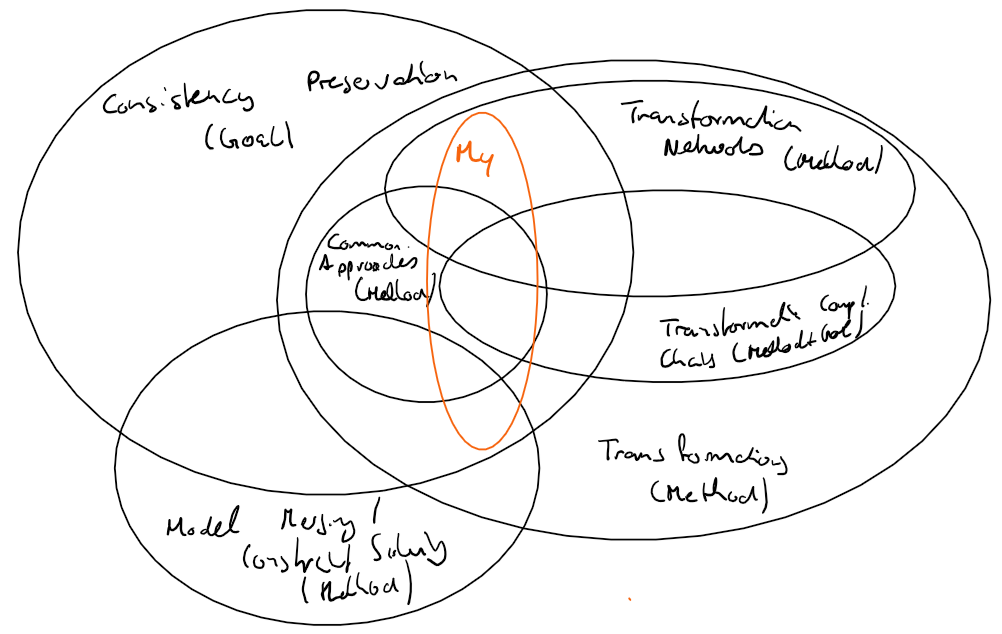
\includegraphics[width=\textwidth]{figures/epilogue/relatedwork/research_areas.png}
    \caption[Overlaps of related research areas]{Sketch of different research areas (circles) related to the work of this thesis, their overlaps, and the relation to contributions of this thesis (shaded red).}
    \label{fig:relatedwork:areas}
\end{figure}

\mnote{Relations of topics}
\autoref{fig:relatedwork:areas} depicts an overview of the topics and research areas that we relate our work to and sketches how they are related to each other and to our contributions, indicated by overlaps of the ellipses representing them.
The figure is neither complete, nor do the sizes of the areas and overlaps have a specific meaning.
We do also not depict the relation of each of our contributions to related topics in that figure, but do so in the subsequent sections.
Several research topics are cross-cutting, such that some work fits into multiple categories.
We discuss these works in the areas to which they are mostly related.
Parts of the discussions in this chapter have already been published in previous work~\owncite{klare2018docsym, klare2019icmt, klare2019models, klare2020compatibility-report, klare2021Vitruv-JSS}.


%%%%
%% CONSISTENCY AND ITS PRESERVATION
%%%%
\section{Consistency and its Preservation}

\mnote{Generality of consistency}
Checking and preserving consistency of software artifacts, i.e., models, has been researched in several contexts.
It covers a broad topic and is often traced back to the \emph{view-update problem}, which considers the backpropagation of changes within a view to the original source and is especially known from database engineering~\cite{bancilhon1981viewUpdate-TDS}.
Consistency has been considered for different development artifacts, including the common scenario of \emph{roundtrip engineering} between \gls{UML} models and code~\cite{dantas2005umlsync-ISPSE}, and especially rose with the definition of a general methodology defined by the \gls{MDA}~\cite{mda} process.
Depending on the scenario, the kinds of dependencies and inconsistencies between multiple models can vary and have been discussed by \textcite{kolovos2008a}. 
Several approaches provide domain-specific solutions for consistency problems, such as for consistency between SysML~\cite{sysml} and AUTOSAR~\cite{scheid2015autosar} in the automotive domain~\cite{giese2010a}.

\mnote{Model consistency approaches}
The development of modeling frameworks, such as the \gls{EMF}~\cite{steinberg2009emf}, have enabled the definition of tools, such as transformation languages, that are independent from the actual metamodels to consider consistency between.
General methods and approaches regarding model consistency have been based on such modeling framework and can be separated into approaches that are only able to check consistency of models~\cite{reder2012incrementalchecking} and those that are also able to preserve or enforce it.
Consistency-preserving approaches range from providing recommendations for repair~\cite{ohrndorf2018repairRecommendataions-ICSE} over generation and classifications of repair options~\cite{kretschmer2018repairDiscovery-ICSE} to approaches that actually perform \emph{model repair}, which have been subject to intensive research and surveyed by \textcite{macedo2017ModelRepairClassification-TSE}.
The survey also classifies approaches regarding their support for the scenario of keeping multiple, i.e., more than two, models consistent, which is the focus of this thesis, and found that only one of the considered approaches is able to handle multiple models, which is done by considering consistency pairwise, like we do in our work.

\mnote{Focus on preservation}
We focus the discussion of related work on consistency preservation rather than checking, as the contributions of this thesis aim to support it.
We first depict a general overview of relevant consistency preservation approaches, including the foundation of the view-update problem, model merging, constraint solving, as well as the methodology of multi-view modeling.


\subsection{The View-Update Problem}

\mnote{View update in databases}
The \emph{view-update problem} is common in software engineering.
It occurs whenever a view, i.e., a model, is supposed to represent information from some underlying source, which in our case is also a model, such that modifications to this view can be propagated back to the underlying source without changing information that is not contained in the view.
The problem was and is a central topic in database research~\cite{bancilhon1981viewUpdate-TDS, dayal1982viewUpdate-TDS}, where views are derived from database tables.
Updating database tables with changes in views to them, denoted as \emph{update translation}~\cite{bancilhon1981viewUpdate-TDS}, can be achieved by considering a \emph{complement} view that contains all information of the database that is not contained in the modified view.
This means that the Cartesian product of the functions for generating a view and its complement must be injective.
Calculating the update of the database after changes to the view can be achieved by inverting this function.
There are many possible complements to a view, but for considering a view \emph{updatable}, it must be possible to translate its 
updates to the database tables with a constant complement~\cite{bancilhon1981viewUpdate-TDS}.
Update translation must, however, ensure that it leaves invariant the information in the complement.
It is thus inevitable to design views and complements properly to enable automated translation of updates.

\mnote{Lenses framework}
An application of the view-update problem to software artifacts and, in particular, to transformations, is given by the \emph{lenses} framework~\cite{foster2005Combinators-POPL, foster2007combinators-TPLS}.
It defines two essential operations, which are \emph{get} for deriving a view from a model and \emph{putback} for propagating changes in the view back to the model.
This defines a transformation between a view and an underlying model.
Specific laws ensure that lenses are \emph{well-behaved}~\cite[Def.~3.2]{foster2007combinators-TPLS}, i.e., that they are complete such that all information changed in a view is propagated back to the model, and that they do not perform unintended changes.
The proper design of the \emph{putback} function influences expressiveness and robustness of the view and the changes that can be propagated back to the underlying source~\cite{foster2007combinators-TPLS}.
Lenses depict a well-researched formal foundation to express and study incremental transformations~\cite{stevens2008bxalgebraic-ICGT}.

\mnote{Delta lenses}
While lenses %and the view-update problem in database research %, as well as the view-update problem in database research, 
originally consider states of models, \emph{delta lenses}~\cite{diskin2011StateToDeltaSymmetric-MODELS} consider the application to deltas, which conforms to our notion of changes and consistency preservation according to \autoref{def:consistencypreservationrule}.
They particularly consider the so called \emph{symmetric} case~\cite{diskin2011StateToDeltaSymmetric-MODELS}, in which the view is not a projection from the underlying source, but the view and the underlying source are both models with information that is unique to each of them and thus transformations are defined in both directions.

\mnote{Multiary lenses}
Lenses have also been extended to the multiary case, in which more than two models need to be kept consistent~\cite{diskin2018MultiModelSynchronization-FASE}.
It especially reflects that transformations may need to change the originally modified models as well, which is denoted as \emph{reflective updates} in that work and which we have also motivated and introduced with the notion of \emph{synchronizing transformations} in \autoref{chap:synchronization}.
Despite these multiary lenses, work on lenses is especially focused on or related to bidirectional transformations, which build the basis for our work of constructing networks of them.


\subsection{Traceability and Model Merging}

\mnote{Checking consistency}
Traceability is an important concept for different concerns, ranging from comprehension over change impact analysis to the identification and resolution of inconsistencies.
For example, architectures based on correspondence models to identify that elements belong together and affect each other among changes have been developed~\cite{szabo2013traceabilityConsistency-ASWEC}.
While traces are also used as auxiliary or witness structures for consistency preservation, much work on traceability is focused on consistency checking, such as UML/Analyzer~\cite{egyed2006umlanalyzer-ICSE} for checking consistency of \gls{UML} models incrementally, and its generalization Model/Analyzer~\cite{egyed2011modelanalyzer-TSE} for checking consistency of arbitrary models.
These tools were also extended to repair inconsistencies with repair actions derived from the incremental consistency checks to determine the scope of consistency repair~\cite{reder2012resolvingInconsistencies-ASE}.
Our approaches go beyond consistency checking and use traceability especially as a means to trace consistency relations in the practical approach realization to be able to update them among changes.

\mnote{Merging corresponding elements}
Model merging goes beyond traceability by not only providing correspondences for related information, but by merging elements that share and redundantly represent information.
This process is also known as \emph{amalgamation}~\cite{koenig2017efficientConsistencyChecking-ECMFA}.
Model merging consists of matching elements that represent the same information and merging them~\cite{koenig2017efficientConsistencyChecking-ECMFA}.
Such an approach has also been applied in a framework based on category theory~\cite{diskin2010overlapsHeterogeneous-MDI}.
Model merging is comparable to the \commonalities idea (see \autoref{chap:improvement}), as it is also concerned with finding elements that represent the same information. 
Model merging is, however, usually used for merging models into a single, redundancy-free and thus inherently consistent representation or for checking consistency during the merge task, but not to preserve consistency like we do with the \commonalities approach.
In addition, \commonalities relate redundant elements by construction, i.e., as soon as an element is created that requires a corresponding one in another model, it is created, whereas model merging identifies redundant elements after their creation. %Thus \commonalities can be seen as an a-priori approach whereas model merging is an a-posteriori approach for tracing redundancies.


\subsection{Multi-View Modeling}

\mnote{Consistency challenge}
Multi-view modeling, as introduced in \autoref{chap:foundations:multiview}, concerns the description of a system by means of multiple views, reflecting different interests.
A recent survey of such approaches~\cite{cicchetti2019multiview-SoSym} has identified lacking consistency management as a central challenge of them, which is also emphasized by \textcite{reineke2019ProblemMultiView-SoSym}.
In addition to identifying this challenge, \textcite{persson2013characterizationMultiView-EMSOFT} classify different types of relations between views to be distinguished.
Our contributions can be applied in the context of multi-view modeling, as model transformations are a possible means to solve the consistency challenge in multi-view modeling.
We give an overview of different approaches to multi-view modeling, even beyond transformations, to sketch the research field and embed and highlight the relevance of our contributions.

\mnote{Orthographic software modeling}
A systematic approach to multi-view modeling is \gls{OSM} (see \autoref{chap:foundations:multiview:osm}).
It considers the description of a system in a single repository, a \gls{SUM}, from which views are projected that allow modifications that can be propagated back to the \gls{SUM}.
The approach defines how views can be organized in orthographic dimensions representing the different concerns that shape a view.
The idea is comparable to a hybrid approach using an underlying metamodel from which multiple views can derived~\cite{cicchetti2012hybridMultiView-EASST}, which are consistent through the underlying model by construction.
A \gls{SUM} can be achieved by construction or by applying data integration approaches~\cite{angel2018integration-CLSS}.

\mnote{SUM approaches}
Different ways to construct a \gls{SUM}, i.e., an underlying repository of consistent information, have been discussed and classified~\owncite{meier2019modelsward,meier2020ccis}.
\vitruv, which we have introduced in \autoref{chap:foundations:multiview:vitruv}, composes a \gls{SUM} from different models, which conform to metamodels of existing tools and are kept consistent by transformations, and calls this a \vsum.
Role-oriented single underlying models (R-SUMs) let model elements take different roles by separating their properties into different \emph{compartments}, such that depending on the view someone takes on the system only specific compartments are relevant~\cite{werner2018rsum-SEAA, werner2018rsum-MRT}.
They provide \emph{relation compartments} that can be used to relate information of multiple elements to preserve their consistency.
\textsc{MoConseMi} constructs a \gls{SUM} by metamodel integration~\cite{meier2019MoConseMi-Models}.
It can be considered a model merging approach, which does not only merge the models but also the metamodels by means of operators that check and preserve consistency.
While all these approach rely on the idea of multi-view modeling and project views from a single repository, they all ensure consistency of information in the underlying repository in different ways by means of some explicit consistency preservation mechanisms, be they called transformations, operators or something else, such that they all have to deal with the challenges that we have addressed in this thesis.
\emph{Action-driven consistency}~\cite{ali2020ActionDrivenConsistency-SAM} is a comparable approach, which uses language-specific actions rather than generic change operations, but is, in fact, only a framework for defining transformations with actions of language-specific semantics.

\mnote{Collaborative multi-view modeling}
In general, multi-view modeling considers that one or multiple users work on a single system with different interests reflected by different views.
A realization of multi-view modeling with a specific focus on collaborative engineering is the \emph{DesignSpace} approach~\cite{demuth2015designSpace-SAC,egyed2019consistencyArtifacts-Computer}, which integrates the previously discussed Model/Analyzer approach for checking consistency.
It is comparable to a \vsum approach, but performs an ad-hoc integration of data and definition of consistency repair rather than applying predefined relations and preservation rules as a \vsum in the \vitruv approach does.
The DesignSpace approach even integrates consistency preservation capabilities~\cite{troels2019liveconsistency-SAC, khelladi2019sideeffects-SLE} and especially considers that artifacts may be temporarily inconsistent, as well as that inconsistencies have to be resolved in potentially complex processes~\cite{kretschmer2020ConsistentChangePropagation-SoSym}.

\mnote{Multi-paradigm modeling}
\emph{Multi-paradigm modeling}~\cite{vangheluwe2003mpm-WSC} covers an idea that is comparable to multi-view modeling.
It aims at combining multiple modeling formalisms with transformations to avoid redundant specification effort and inconsistencies, with a particular focus on engineering domains beyond software engineering.
In consequence, it also focuses on the runtime state of continuous and hybrid systems rather than the static structure of discrete systems, and is especially concerned with simulations of a system.
Current research especially applies it in the context of cyber-physical systems~\cite{carreira2020mpm4cpsfoundations}.
Multi-paradigm modeling covers the broad topic of model consistency, especially for cyber-physical systems design, and relies on foundations such as transformations and the construction of networks of them, such that is serves as an application area of our contributions, like multi-view modeling does.
%Especially focused on multiple interests regarding a single system, rather than collaboration.

\mnote{Macro- and megamodeling}
\emph{Macromodeling} denotes a methodology~\cite{salay2012macromodelingMethodoloy-MODELS} for defining relations between multiple models for different purposes, ranging from only improving comprehension to consistency management~\cite{salay2008macromodeling-ASE,salay2009macromodels-CAiSE}.
It is comparable to the notion of \emph{megamodels}, which reflect systems of models, and relations, properties and operations over them~\cite{diskin2013megamodeling-SLE}.
To express relations between models, the application of collection-based operators known from functional programming have been investigated~\cite{salay2015megamodeling-MODELS, salay2020megamodeling-SoSym}.
\Citeauthor{stevens2020BuildingFromMegamodels-SoSym} applies megamodel terminology to transformation networks~\cite{stevens2020BuildingFromMegamodels-SoSym}, which we discuss in more detail regarding transformations and networks of them.

\mnote{Conclusion}
Most multi-view modeling approaches, if considering consistency between multiple models and its preservation at all, assume that there is a common knowledge about how all involved models shall be related.
When knowledge about relations between views is distributed, like we assume for the construction of transformation networks, and thus the relations between views are defined independently, the problems such as incompatibilities discussed in this thesis can occur. 
In consequence, regardless of the multi-view modeling approach, the findings of our work are relevant for most of these approaches.
Multi-view modeling, including multi-paradigm modeling and \gls{SUM} approach, are thus an important application area of our contributions.


\subsection{Constraint Solving and Model Finding}

%While constraint solving is an approach to describe models as logic terms and try to find a consistent result by solving constraints, constraint solving is also important for us in regards to the compatibility approach, which verifies OCL statements, which is also a constraint solving approach.

\mnote{ASP}
Some approaches consider consistency preservation as a constraint solving problem rather than a transformation problem.
They use constraints to represent consistency relations, like we do for the relations of transformations, and then try to find valid solutions after modifications that introduce inconsistencies by model finding.
\gls{ASP}~\cite{cicchetti2006asp-EDOCW,eramo2008asp-EDOCW} is an approach based on logical programming techniques.
Logic programs define the rules and constraints for models, such that consistent models are those fulfilling all of them, which are known as \emph{ground instantiations}.
After changes, the \gls{ASP} engine can deduce consistent sets of models reflecting the given changes and the original states of the models.
%We, however, focus on transformation-based techniques to maintain consistency and issues related to that, which is why we point out constraint solving techniques for consistency management another research directions but do not discuss that research area in more detail.

\mnote{Echo}
\emph{Echo}~\cite{macedo2013echo-ASE} is a model repair tool that checks and resolves inconsistencies by model finding.
It employs \emph{Alloy}, which is a formal specification language supporting model finding via constraint solving.
It can transform Ecore models, as well as \gls{OCL} expressions, \gls{QVTR} transformations and \gls{ATL} transformations into Alloy descriptions~\cite{macedo2013qvtrAlloy-FASE, macedo2016qvtAtlAlloy-SoSym}, which applies constraint solving to validate consistency and finds options to restore it.

\mnote{Conclusion}
Constraint solving is a different approach to consistency preservation than transformations, as it relies on declarative specifications of consistency and employs generic solvers to find solutions for inconsistent models.
A benefit of using transformations is that they provide more means to influence how consistency is actually achieved.
Constraint solving, however, can inherently deal with an arbitrary number of models, as constraints are not restricted to two models, whereas the imperative specification in transformations how consistency between models is restored becomes difficult for more than two models.
%Thus, constraint solving provides a different approach to solving the underlying problem of model consistency.
Since we focus on transformation-based techniques, we depict constraint solving as an alternative technique for consistency preservation, but do not discuss that research area in mode detail.
In addition, it serves as a foundation of our approach for identifying compatibility, in which we use constraint validation techniques.



%%%%
%% CONSISTENCY BY MODEL TRANSFORMATION
%%%%
\section{Consistency by Model Transformation}

\mnote{Transformations between multiple models}
We have focused on model transformations as a means to preserve consistency between multiple models, as transformations provide a high degree of freedom for specifying how consistency is preserved.
Most existing transformation approaches are restricted to the bidirectional case~\cite{weidmann2020ApplyingBidirectionalTransformations-WSRE, cleve2019dagstuhl}, keeping two models consistent.
Two central approaches for relating multiple metamodels by transformations are transformation networks and multidirectional transformations.
They have been discussed in a dedicated Dagstuhl seminar~\cite{cleve2019dagstuhl} with a particular focus on the usage of networks of bidirectional transformations and the interaction of several such transformations.
%Working groups investigated scenarios, in which networks of bidirectional transformations do not suffice and thus validated our assumption in \autoref{chap:correctness:notions_consistency:monolithic_modular}.

\mnote{Relevant transformation approaches}
We have identified multidirectional transformations to be complex to specify, whereas networks of bidirectional transformations have limited expressiveness~\cite{stevens2020BidirectionalTransformationLarge-SoSym}, which, however, may not be practically relevant~\cite{cleve2019dagstuhl}.
Adding auxiliary models circumvents the limitations of binary relation expressiveness in transformation networks~\cite{stevens2020BidirectionalTransformationLarge-SoSym}, like we do with the \commonalities approach.
Research on transformations is especially driven by theoretic investigations of bidirectional transformations and tools that support their specification.
Since reasonable consistency preservation requires incrementality, the area of incremental, bidirectional transformations is most relevant for that purpose.
Different scenarios regarding the transformation direction and the scope of changes that need to be propagated between two models have been classified and based on a taxonomy~\cite{diskin2016Taxonomy-JSS}.
Since our approaches do not make any restrictions regarding the transformation directions or the scope of changes to be considered, our contributions fit into any of the needs for consistency preservation covered by this classification.


\subsection{Bidirectional Transformations}

\Citeauthor{stevens2018bidirectionality-ECMFA} emphasizes the importance of bidirectionality for model transformations and for software engineering in general~\cite{stevens2018bidirectionality-ECMFA}.
Although bidirectional transformations themselves are not sufficient for achieving consistency between more than two models, they are still relevant for and related to our work.
First, we compose networks of transformations out of bidirectional transformations, thus they serve as a foundation for our work.
Second, some approaches already implement necessities for building transformations networks, for example by matching existing elements to achieve synchronization, like provided by \gls{QVTR}.
Bidirectionality can be achieved by an explicit specification of consistency preservation in both directions, for example with imperative languages such as \gls{QVTO}~\cite{qvt}, by the specification of one direction and inference of the opposite one~\cite{xiong2007backwardTransformation-ASE, hettel2008synchronization-ICMT, semerath2016backwardTransformation-MODELS}, or by declaratively specifying constraints that have to hold and inferring the way to preserve it in both directions, like with \gls{QVTR}.

\mnote{Properties}
Bidirectional transformations are a well-researched option for keeping two models consistent.
They have been formally founded on the lenses framework~\cite{stevens2008bxalgebraic-ICGT}, whose laws have been related to requirements of bidirectional transformations, such as correctness, hippocraticness or undoability~\cite{stevens2010sosym}.
Correctness and hippocraticness have been identified as essential properties for bidirectional transformations, whereas undoability is beneficial but usually not achievable~\cite{stevens2010sosym}.
We have reflected correctness and hippocraticness in our formalization (see \autoref{def:consistencypreservationrulecorrectness} and \autoref{def:hippocratictransformation}).
Another interesting property is the one of \emph{least change}, which we have discussed in \autoref{chap:orchestration} as an improvement for finding orchestrations.
This property has been considered as a basic principle~\cite{cheney2017LeastChangeBx-JOT} especially by transformation tools~\cite{macedo2016qvtAtlAlloy-SoSym}.
\textcite{stevens2012equivalences-EASST} also discusses equivalence relations given by the consistency relations of bidirectional transformations, denoting those instances of one metamodel that are consistent to the same instances of another.
They can be considered as an explicit description of different options for a transformation to select from, as discussed in \autoref{chap:orchestration}.

\mnote{Transformation languages overview}
Several tools and languages have been developed to support the specification of bidirectional transformations, which have been summarized and classified over the time in several surveys regarding different criteria~\cite{stevens2008LandscapeBidirectionalTransformation-GTTSE, diRuscio2012transformations-SFM, kusel2013SurveyIncrementalTransformation-ME, jakumeit2014transformationTools-SCP, samimi-dehkordi2015bidirectionalSynchronization-ICCKE, samimi-dehkordi2016iccke,hidaka2016classificationTransformations-SoSym,kahani2019SurveyTransformationTools-SoSym}.
It is a current and open discussion whether specific transformation languages actually provide benefits over using general-purpose languages for specifying model transformations, especially because of lacking evidence and adoption~\cite{burgueno2019futureTransformationLanguages-ICMT}. 
For our work, it is, however, not important whether a transformation language or a general-purpose language is used to define a transformation, since we only define and consider the properties a transformation has to fulfill, no matter how it is defined.
Thus, our contributions are not tied to specific languages or the usage of transformation languages at all.

\mnote{Transformation languages details}
Popular approaches for specifying bidirectional transformations include imperative and declarative languages, such as the \gls{QVT}~\cite{qvt} language family, the \gls{ATL}~\cite{jouault2006a,xiong2007backwardTransformation-ASE} and especially an incremental realization of it~\cite{martinez2017incrementalATL-SCP}, the Epsilon languages~\cite{kolovos2014epsilon-Book} and approaches using them~\cite{samimi-dehkordi2018evlStrace-IST}, as well as \gls{VIATRA}.
\gls{VIATRA}~\cite{bergmann2015viatra-ICMT, varro2016viatra-SoSym} is a consistency framework based on an event-driven mechanism, which conforms to our notion of delta-based consistency preservation (see \autoref{def:consistencypreservationrule}) and which the authors refer to as \emph{change-driven} transformations~\cite{bergmann2012changeDriven-SoSym}.
A different kind of specification is followed by graph-based approaches, such as \glspl{TGG}, which were originally developed by \textcite{schuerr1995a} and which are well-suited for model transformations~\cite{anjorin2014EfficientSynchronizationTGG-ECMFA}.
Several tools for specifying \glspl{TGG} have been developed~\cite{leblebici2014IncrementalTGGSurvey-GTVMT}, in particular based on the \gls{EMF}, such as eMoflon~\cite{anjorin2014diss}.
Expressiveness~\cite{anjorin2012complexManipulationTGG-BX} and applicability of \glspl{TGG} are continuously extended, e.g., in terms of applying integer linear programming to consider consistency as an optimization problem~\cite{weidmann2019TGGandILP-SLE,weidmann2020TGGsAndILPSchemaCompliance-FASE}.
\Citeauthor{kramer2017a} has proposed an approach combining a language for declarative mappings between metamodels with a fallback language for imperative consistency repair~\ownandothercite{klare2016b}{kramer2017a}, which have been developed for the \vitruv framework~\owncite{klare2021Vitruv-JSS}.
We have used these languages for the realization of the \commonalities languages and for evaluation purposes throughout this thesis.
While all these languages are external \glspl{DSL}, i.e., they use an own syntax, some languages~\cite{buchmann2018bxtend-Modelsward, hinkel2019internalTransformation-SoSym} are internal \glspl{DSL}, i.e., they reuse existing languages by providing an internal \gls{API} and are thus more lightweight.

\mnote{Conclusion}
Extensions to support consistency preservation between more than two models have been proposed for only few tools, which we discuss subsequently.
In general, our approaches to build transformation networks can be applied to any existing approach or language for bidirectional transformations.
Depending on which assumptions a language makes and which abstraction it provides, different requirements to fulfill our notion of synchronizing transformation have to be considered.
First, most languages operate in a state-based manner and thus applying a change to a modified state can be more complex than in a delta-based approach, in which changes can be reapplied to another state of the models. 
In such a case, approaches for change reconstruction have to be applied, which are especially difficult to develop for textual languages such as code~\cite{falleri2014codeDifferencing-ASE}.
Second, most languages do not allow the definition of synchronizing transformations (see \autoref{def:synchronizingtransformation}), such that our approach for making transformations synchronizing proposed in \autoref{chap:synchronization} has to be applied, whereas some languages, such as \gls{QVTR}, already provide a level of abstraction that achieves synchronization.


\subsection{Synchronizing Transformations}

\mnote{Concurrent synchronization}
Transformation networks of arbitrary topology require synchronizing transformations (see \autoref{def:synchronizingtransformation}), as a special case of bidirectional transformations.
In our definition, this covers transformations that consider changes to both models and are able to update both of them.
While in literature the term \emph{concurrent synchronization} always covers this scenarios, the term \emph{model synchronization} is used ambiguously for incremental updates only~\cite{giese2009incrementalModelSynchronization-SoSym}, as well as for concurrent synchronization~\cite{samimi-dehkordi2015bidirectionalSynchronization-ICCKE}.
Thus, much work on model synchronization is not related to the concurrent modification scenario that we consider.
The case of interest is also denoted as \emph{bidirectional synchronization with reconciliation}~\cite{antkiewicz2008synchronizationDesignSpace-GTTSE}.
Work in this area is especially related to our work on synchronization, as presented in \autoref{chap:synchronization}.

\mnote{EVL+trace}
\emph{EVL+trace}~\cite{samimi-dehkordi2015bidirectionalSynchronization-ICCKE} considers concurrent modifications of both models related by a transformation.
The authors make a case distinction of several scenarios of concurrent changes to support the developer of transformations in considering these different situations of concurrent modifications.
They do, however, leave it up to the developer to implement the scenarios.
In addition, they consider the case of conflicting user changes, which we have excluded in this thesis as it is not relevant during the execution of a transformation network if transformations are not conflicting, thus making the necessary solution that we have proposed in \autoref{chap:synchronization} simpler.

\mnote{TGG approaches}
Approaches for handling concurrent modifications to both models are often concerned with the case of conflicts, i.e., that changes concurrently performed in both models are conflicting.
This has, for example, been researched for \glspl{TGG}~\cite{hermann2012concurrentSynchronization-FASE, orejas2020IncrementalConcurrentSynchronization-FASE, weidmann2020ConcurrentSynchronization-SLE}.
\textcite{orejas2020IncrementalConcurrentSynchronization-FASE} proposed an approach that provides different solutions to synchronize concurrent modifications and leaves it up to the developer to decide how conflicts shall be resolved.
While this behavior may be desired and beneficial for resolving conflicts of user changes, having multiple transformation results is not applicable in transformation network as the execution has to proceed with a single one.
\textcite{weidmann2020ConcurrentSynchronization-SLE} propose an approach based on integer linear programming to find consistent solutions after concurrent updates.
This approach also handles conflicting changes and could thus be applied in transformation networks to resolve conflicting user inputs.
It should, however, not replace the approach we have presented for the synchronization case in transformation networks, as performing the matching of existing elements by construction through encoding it into transformations ensures that matching is performed deterministically and successfully rather than potentially getting unexpected results when considering the scenario as an optimization problem solved by integer linear programming.

\mnote{Merging unidirectional execution}
One highly related approach to synchronize concurrent changes with bidirectional transformations is given by \textcite{xiong2009parallelUpdates-ICMT,xiong2013SynchronizingConcurrentUpdates-SoSym}.
They propose a special process of executing a transformation in both directions and merging the generated changes in between with a special three-way merger.
While the idea of executing the consistency preservation rules on specific states of the two modified models to reflect concurrent changes is equal to our synchronization approach presented in \autoref{chap:synchronization}, there are two essential differences.
First, their approach merges the changes rather sequentially applying them.
Second, their approach does not iteratively apply the preservation rules in both directions to improve partial consistency but assumes to achieve consistency after executing each of them once. Thus, they do not consider that changes to one model may require both models to be changed.
Merging the changes rather than sequentially applying them has the benefit of not requiring the transformation developer to ensure that elements are not created multiple times. However, the merger must correctly consider that case, which, in general, can only be implemented as a heuristic.
The differences between our and the discussed approach especially arise from their different goals. 
While our approach aims to synchronize concurrent changes performed by transformations, which will not produce conflicts if the transformations are not contradictory, their approach merges user changes, because these changes can, of course, be conflicting and these conflicts need to be resolved.

\mnote{Design Patterns}
Design patterns are an established way of defining a common notion for solutions to recurring problems, such as the design patterns for object-oriented software by \textcite{gamma1995designPatterns-Book}.
We have also defined patterns to achieve synchronization of transformations, and several further patterns have been researched for the specification of transformations.
This especially comprises patterns for specific kinds of consistency relations~\cite{iacob2008a} and the improvement of modularization~\cite{lano2014a}.
Patterns for transformations have been surveyed by \textcite{lano2018a}, and even ways to semi-formally describe them have been proposed~\cite{ergin2016patternsTransformations-CLSS}.
These patterns focus on improving the development of single transformations and mainly unify how specific kinds of consistency relations can be expressed in transformation languages, but they do not aim to achieve interoperability with other transformations like the patterns that we have proposed do.
However, the catalog of \textcite{lano2014a} also comprises patterns for the single instantiation of elements, like we have discussed for achieving synchronizing transformations, but covers a more general use case than the specific scenario of ensuring synchronization of a transformation in a transformation network.


\subsection{Transformation Networks}

\mnote{Combining transformations}
Combining multiple transformations, in particular bidirectional transformations, to a network is one approach to preserve consistency between multiple models.
\Citeauthor{laemmel2004coupledTransformations-WSET} has already emphasized the necessity to couple transformation early in the research of model transformations in \gls{MDSD}~\cite{laemmel2004coupledTransformations-WSET}.
Combining transformations to networks is a task that is external to the individual transformations and languages to define them, which is why existing transformation languages do not consider the combination of transformations developed with them.
\textcite{stevens2020BidirectionalTransformationLarge-SoSym} states that it is reasonable to target consistency between multiple models by combining binary transformations, even though multiple binary relations cannot express all relations between multiple models.
She also derives the relaxed notion of \emph{binary-implemented} relations, which requires that models consistent to the binary relations need to be consistent to the multiary one, but not vice versa.

\mnote{Networks vs. multidirectional transformations}
Favoring transformation networks over multidirectional transformations is motivated by multiple reasons.
Networks are easier to develop when domain knowledge is distributed~\owncite{klare2018docsym}, and they are easier to comprehend by a single developer~\cite{cleve2019dagstuhl, stevens2020BidirectionalTransformationLarge-SoSym} in comparison to multidirectional transformations.
Additionally, binary transformations are researched well and a variety of tools supporting different kinds of specifying them exist, as discussed in the previous subsection.
Finally, there is also the problem of technical debt in transformations~\cite{lano2018technicalDebt-ICMT}, which can be mitigated by modularizing the specification rather than developing a monolithic multidirectional transformation.
Research regarding transformation networks especially concerns the orchestration and execution of them and is thus related to our work on orchestration, which we have presented in \autoref{chap:orchestration}.

\mnote{Orchestration approaches}
Several research papers consider theoretical properties of transformation networks, especially including their resolvability, i.e., the possibility to find a consistent orchestration.
While we aim at finding a \emph{universal} approach for orchestrating and executing transformations of arbitrary transformation network topologies, most existing approaches restrict the number of allowed executions.
A general approach for a platform managing multiple models~\cite{denton2008naomi-Models} considers change propagation based on a dependency graph between the models and performs a depth-first search for determining an execution order.
In networks of arbitrary topology, however, no such explicit dependencies exist, and the approach is restricted to executing each transformation only once.
Likewise, \textcite{dirocco2017ConsistencyRecoveryInteractive-MODELS} describe a simple strategy for orchestrating transformation networks, but also make strong assumptions in terms of the necessity to apply each transformation only once.
\textcite{stevens2020BidirectionalTransformationLarge-SoSym} proposes a strategy that also executes each transformation only once in one direction. This includes a notion of authoritative models, which are not allowed to be changed, and does not consider synchronizing transformations.
She also discusses non-termination and resolvability issues, i.e., reasons for not finding a consistent orchestration, which can arise from incompatibilities of the relations, as we have discussed in \autoref{chap:compatibility}, or further problems such as the selection of different options, as we have discussed in \autoref{chap:orchestration}, but that work is restricted to the single execution of each transformation and does not distinguish and discuss the reasons for missing resolvability like we do.
In the same way, \textcite{stevens2020BuildingFromMegamodels-SoSym} proposes to find an \emph{orientation model} that defines in which direction transformations are executed after a change to restore consistency, also considering authoritative models.
If there are, however, several transformations that modify the same model, this work leaves it up to the developer to ensure that the transformations are executed in an appropriate order such that all consistency relations hold afterwards.
We have presented use cases in which this is too limiting to be used as a universal approaches for orchestration, which is why our approach for orchestration presented in \autoref{chap:orchestration} explicitly considers that an arbitrary number of transformation executions may be necessary.

\mnote{Provenance}
Provenance is a topic of growing attention and importance in research for bidirectional transformations~\cite{cleve2019dagstuhl,anjorin2019provenance-tapp}.
While \textcite{anjorin2019provenance-tapp} especially consider provenance information about changes performed by a single transformation, we provide such information for the cause of a failure of a transformation network.
This affects and supports the network developers rather than the users of a transformation.

\mnote{Reuseability}
One motivation for building transformation networks and our assumptions is the modular reuse of individual transformations.
There has been research regarding the reuse of and variability in transformations~\cite{bruel2020transformationReuse-SoSym}, supporting the derivation of different transformations from a single specification for different purposes, comparable to product lines.
An approach for transformation product lines reuses concepts from software product lines~\cite{delara2018transformationProductLines-Models} to derive several transformations with variable parts from one specification.
Another approach supporting reuse considers that it is not necessary to define a transformation for two metamodels, but only for some requirements that two metamodels have to meet~\cite{delara2019transformationResue-TOSEM}, thus allowing reuse of a transformation for all metamodels fulfilling these requirements.
Such approaches for reusability support development processes that support the assumptions that we have made in our work.
Although these works consider quality properties of transformations, such as reuse, which we have discussed in \autoref{chap:classification}, they are not concerned with quality properties of a transformation network and especially the reuse of transformations in other network.


\subsection{Transformation Composition and Chains}

\mnote{Composition techniques}
Transformation composition has especially been researched in terms of creating chains of transformations, composing larger transformations from smaller ones, and finding and extracting common parts in different transformations, known as \emph{factorization}.
These approaches deal with specific problems of the execution of and compatibility in transformation networks and are thus related to our work on compatibility and orchestration, which we have presented in \autoref{chap:compatibility} and \autoref{chap:orchestration}.

\mnote{Transformation chains}
A transformation chain defines a sequence of transformations to represent an \gls{MDSD} process.
It especially covers the case that an abstract model at a high level of abstraction is to be transformed into a model at a low level of abstraction across one or more other models at different abstraction levels, comparable to the idea of the \gls{MDA} (see \autoref{chap:foundations:modeling:mdsd}).
Transformation chains thus deal with specific kinds of transformation networks.
While approaches for transformation chains have in common that they support the specification of such chains, often with dedicated languages, they aim to achieve different additional goals.
Tools like UniTI~\cite{vanhooff2006a, vanhooff2007UniTI-MODELS, pilgrim2008constructingChains-ECMDA} enable the explicit specification of chains while treating models as black-boxes, FTG+PM~\cite{lucio2013FTGPM-SDL} provides a complete framework that also aims to model and support processes of applying transformation chains, and CITRIC~\cite{basciani2018chains-MODELS} especially aims to optimize the automatic selection of transformation chains between two defined metamodels.
Transformation chain approaches are currently also applied to low-code development platforms~\cite{sahay2020TransformationCompositionLowCode-Models}.
However, tools like UniTI derive compatibility from additional, external specifications of the transformations, for which conformance to the actual transformations is not guaranteed.
Additionally, transformation chains are only a special case of transformation networks, as each transformation network is also aware of the individual transformation chains between all pairs of metamodels.
They are, by construction, not that prone to correctness issues, because there are no multiple paths of transformations that can lead to cycles and conflicts in the network, like was our motivation for the \commonalities approach in \autoref{chap:improvement}.

\mnote{Properties of chains}
To improve maintainability, approaches for separating transformation chains into smaller concern-specific ones~\cite{yie2012a} and to support evolution~\cite{yie2009a} have been developed.
Other approaches support the incremental development by automated testing~\cite{kuester2009incremetalChainDevelopment-MODELS}.
\Citeauthor{etien2010Combining-SAC} consider specific properties of transformation chains.
They investigate how two transformations with incompatible input and output metamodels can be chained~\cite{etien2010Combining-SAC}, and how conflicts in terms of results depending on the execution order can be detected~\cite{etien2012Chaining-AMT}.
A comparable approach validates whether chained transformations fit together in terms of matching contracts and types during both construction and execution~\cite{heidenreich2010compositionTransformations-ICMT}.
Although these approaches are related to finding interoperability issues and to finding an orchestration for transformations, they particularly aim at checking syntactic compatibility rather than semantic interoperability leading to termination with consistent results, and they do not aim to relieve developers from the task of finding an execution order manually, like we do in our work.

\mnote{Transformation composition}
A variety of transformation composition approaches is focused on composing transformations between the same two metamodels.
They can be separated into internal and external techniques~\cite{wagelaar2008a}.
Internal techniques are white-box approaches integrated into a language~\cite{wagelaar2011a}, such as inheritance or superimposition techniques~\cite{wagelaar2010a}.
External approaches consider the transformations as black-boxes and thus work independently from the language. 
Our approaches can be considered as a combination of white-box and black-box approaches.
Achieving synchronization is an intrusive concept that needs to be applied to the implementation of a transformation, thus it is a white-box approach to the transformation.
Analyzing compatibility requires knowledge about the relations encoded in the transformations, thus it is not a white-box approach, as it does not consider the actual consistency preservation rules. Considering the consistency relations as a kind of interface, we may denote the compatibility analysis as a gray-box approach.
Finally, the orchestration of a transformation network works under the assumption a having synchronizing, compatible transformations, which are then orchestrated without considering their contents, thus using a black-box approach.
The proposed \commonalities approach specifies how to define the internals of transformations and thus represents a white-box approach.

\mnote{Transformation modularization}
Factorization approaches identify common parts of transformations and extract them into a base transformation from which the individual parts are extended~\cite{cuadrado2008a}.
Such approaches use intrusive operators that adapt the transformations for composition, whereas we only provide construction approaches and non-intrusive analyses, but do not perform intrusive modifications of the transformations.
A recent approach applies higher-order transformations to modularize transformations~\cite{fleck2017transformationModularization-TSE}.
Some approaches also deal with processes for specifying composition, which simply assume interoperability of the individual transformations~\cite{oldevik2005a}.

\mnote{Interoperability and maintainability}
Existing composition approaches especially have the goal of enhancing modularization of transformations to improve maintainability and reusability, and thus support composition of transformations between the same metamodels. 
We, in contrast, combine transformations between different metamodels and with the goal of achieving interoperability rather than maintainability.
However, our findings on compatibility can also be applied to composition of transformations between the same metamodels, as compatibility is also a reasonable and relevant notion for a single transformation, as we have identified in our evaluation in \autoref{chap:correctness_evaluation}.


\subsection{Multidirectional Transformations}

\mnote{Multidirectional approaches}
Multidirectional transformations are an alternative to networks of bidirectional transformations.
Although they benefit from being less prone to interoperability issues, they do not allow for modular definitions of consistency specifications.
Early ideas include the Multi Document Integration (MDI) approach~\cite{koenigs2006MGGs-SoSym}. The approach proposes \glspl{MGG} as an extension of \glspl{TGG} for defining transformation rules between multiple models.
Another extension of \glspl{TGG} to relate multiple models via one multidirectional transformation rather than defining relations between pairs models are Graph Diagram Grammars~\cite{trollmann2015TransformationTGGtoMultiModel-ICMT, trollmann2016SynchronizationTGGtoMultiModel-ICMT}.
The \gls{QVTR} standard~\cite{qvt} provides multidirectional transformations by design, but \textcite{macedo2014FrameworkMultiDirectional-BX} reveal ambiguities in the standard leading to several limitations of its applicability  and propose strategies to circumvent them.

\mnote{Relation to assumptions}
In contrast to our work, these approaches support the specification of multiary relations between multiple, i.e., more than two, metamodels.
Although this allows to preserve consistency between multiple models and although a single multidirectional transformation is, by design, especially less prone to the correctness and compatibility issues discussed in this thesis, it does not support the specification and preservation of consistency under the assumption of distributed knowledge, requiring independent development and modular reuse, which we have made in this thesis to support the motivational process.
Multidirectional transformations require a transformation developer to have or acquire knowledge about and be able to express all relations between the involved metamodels.
Such approaches may, however, be used to define multidirectional transformations between some of the involved metamodels to be later combined with others to a network.
We have depicted the extension of our approaches to construct transformation networks of multidirectional rather than bidirectional transformation as future work.


\subsection{Commonalities Approaches}

\mnote{Auxiliary artifacts}
Commonalities approaches consider additional auxiliary models in transformation networks, which can be beneficial for different reasons.
These reasons range from expressiveness of multiary relations~\cite{stevens2020BidirectionalTransformationLarge-SoSym,stunkel2018MultimodelCorrespondence-ICPS} to engineering methodologies for improving quality properties, like in this work.
The classification of \textcite{kolovos2008a} covers commonalities models as \enquote{weave models}, which were originally focused on trace models but also apply to the idea of commonalities models.
Work in this area is especially related to our work on the \commonalities approach for improving quality properties of transformation networks, as presented in \autoref{chap:improvement}.

\mnote{Theoretical benefits}
The idea of defining commonalities to express consistency of multiple models was especially researched from a theoretical viewpoint.
Not every multiary relation can be expressed by sets of binary relations~\cite{stevens2020BidirectionalTransformationLarge-SoSym}.
An $n$-ary consistency relation describing consistency between $n$ metamodels can, however, be decomposed into binary relations to an additional $n+1$-th metamodel~\cite{stevens2020BidirectionalTransformationLarge-SoSym}.
Formal foundations for the construction of commonalities have been based on category theory~\cite{stunkel2018MultimodelCorrespondence-ICPS}.
These considerations especially assume one commonalities metamodel, but they may be extended to a hierarchy of them, like we have proposed to use.
These foundations have been used to propose a construction approach of commonalities for comprehensive system~\cite{stunkel2020MultipleModelSynchronization-FASE}.
A formalization of the preservation of multiary consistency relations has been given with the lenses framework~\cite{diskin2018MultiModelSynchronization-FASE}, which was originally proposed by \textcite{foster2007combinators-TPLS} and which we have discussed before.
All this work has a particular focus on expressiveness of consistency relations rather than engineering considerations such as the improvement of quality properties that we focus on.
In addition, if not guaranteeing specific tree structures of commonalities specification, like we have discussed in \autoref{chap:improvement}, a commonalities specification is still a transformation network for which correctness has to be achieved, for example by applying the approaches proposed in this thesis.

\mnote{Domain-specific commonalities}
Some existing approaches to practically use commonalities for keeping multiple models consistent are domain-specific.
The \dually approach~\cite{malavolta2010ADLInteroperability-TSE, eramo2012Dually-SoSym} uses a domain-specific metamodel of commonalities for architecture description languages to which relations of arbitrary architecture description languages can be defined.
\dually is based on a generic model consistency approach, which uses \gls{ASP} based on logical programming techniques.
In contrast to such domain-specific solutions, our \commonalities approach can be applied to arbitrary domains and scenarios.


\subsection{Validation and Verification}

\mnote{Validation as cross-cutting topic}
Validation and verification is important for transformations to ensure that they do what they are supposed to do.
It is cross-cutting to the topics discussed before, since it is relevant for every kind of transformation or composition of them, which is why it is not explicitly depicted in \autoref{fig:relatedwork:areas}.
Most existing approaches concern correctness of a single transformation rather than correctness of a network of them as we have considered.
They either validate single constraints defined in a transformation or validate a transformation as a whole.
Our approach for proving compatibility can be seen as a validation approach for transformation network correctness.

\mnote{Validation of transformations}
Several approaches for the validation of \gls{OCL} constraints used to define conditions on valid models or to define model transformations exist.
\textcite{kuhlmann2011a} and \textcite{gonzalez2012a} have proposed an approach using SAT solvers to validate the existence of models that fulfill specific \gls{OCL} constraints.
Different approaches for the validation of model transformations have been proposed and surveyed~\cite{calegari2013verificationTransformations-ENTCS,rahim2015SurveyTransformationVerification-SoSym}.
\textcite{cabot2010VerificationInvariants-JSS} derive invariants from transformations for verification purposes, such as to find whether a model that fulfills a transformation rule exists.
Comparably, \textcite{cuadrado2017tse} have proposed an approach to analyze \gls{ATL} transformations for errors in them and to find out whether a source model exists that may trigger a transformation.
Other approaches support testing by model comparison~\cite{kolovos2006transformationTesting-WGIMM}, regression testing by deriving test cases that ensure that changes to the transformation or their incremental execution are correct~\cite{troy2018inferenceTransformations-JSS}, or mutation testing~\cite{troya2015imutationTestingTransformations-ICSTW}.
Rather than using constraint logic for verifying a transformation, an approach by \textcite{azizi2017ContractVerification-ICCKE} verifies correctness of transformations written with the Epsilon Transformation Language (ETL)~\cite{kolovos2014epsilon-Book} using the symbolic execution of the transformation.
Instead of checking a transformation on its own, \textcite{vallecillo2012FormalTesting-FMMDE} have proposed to define a formal specification of transformations against which they can be validated.
This is comparable to a validation approach for contracts of transformations, representing contracts as models to be able to apply model validation techniques~\cite{braga2014consistencyTransformations-SCP}.
Finally, \textcite{buettner2012models} have proposed an approach for proving correctness of \gls{ATL} transformations against pre- and postconditions using \gls{SMT} solvers.
Most approaches use some kind of constraint logic or theorem proving for validating correctness of transformations, which is comparable to our approach of proving compatibility of transformation.

\mnote{Validation of transformation networks}
Our defined notion of compatibility is comparable to correctness notions in the approaches of \textcite{cuadrado2017tse} and \textcite{cabot2010VerificationInvariants-JSS}, as they try to figure out whether a rule can be triggered by any model.
Nevertheless, all these approaches consider correctness of a single transformation, whereas we consider a correctness notion for complete transformation networks.
Only few works, especially on transformation chains, consider validation of transformation networks by means of tests~\cite{bauer2011combiningCoverageChains-ICMT} but not by means of constructive or analytic approaches that we have proposed in this thesis.



% \begin{copiedFrom}{DocSym}

% \section*{From DocSym Overview}
% % MULTI-MODEL CONSISTENCY AS A WHOLE
% \emph{Model consistency preservation}, also referred to as %\emph{model synchronization} or 
% \emph{model repair}, is an active field of current research. 
% Nevertheless, most approaches are restricted to consistency between pairs of models~\cite{stevens2020BidirectionalTransformationLarge-SoSym}.
% The kinds of dependencies between multiple models and types of inconsistencies were discussed by \textcite{kolovos2008a}. 
% A summary and classification of model consistency approaches, also regarding their multi-model support, was presented by \textcite{macedo2015a}.

% % BINARY TRANSFORMATIONS LANGUAGES AND EXTENSIONS
% As stated by \textcite{stevens2020BidirectionalTransformationLarge-SoSym}, it is reasonable to target multi-model consistency by combining binary transformations.
% %Multi-model consistency can also be achieved by combining mechanisms for consistency preservation between pairs of models. 
% Especially incremental model transformation languages %, which update models after changes to restore consistency, 
% can be applied by executing the transformations transitively.
% They were surveyed by \textcite{kusel2013SurveyIncrementalTransformation-ME}, including the \gls{ATL}~\cite{jouault2006a,xiong2007backwardTransformation-ASE}, VIATRA~\cite{bergmann2015viatra} and \glspl{TGG}~\cite{anjorin2014b,anjorin2014c}. 
% For \glspl{TGG}, initial concepts for supporting multiple models were proposed~\cite{trollmann2015TransformationTGGtoMultiModel-ICMT,trollmann2016SynchronizationTGGtoMultiModel-ICMT}. 
% Another transformation-based tool is \emph{Echo}~\cite{macedo2013b}. 
% It is based on \emph{Alloy}~\cite{macedo2013a}, which uses \mbox{QVT-R}~\cite{qvt} and model finding to repair inconsistencies. 
% For \mbox{QVT-R}, challenges and steps towards supporting transformations between multiple model were discussed~\cite{macedo2014FrameworkMultiDirectional-BX}.
% \citeauthor{kramer2017a} proposed an approach combining a language for declarative mappings between metamodels with a fallback language for imperative consistency repair~\ownandothercite{klare2016b}{kramer2017a}, developed in the context of the \vitruv framework~\cite{kramer2015a}. %, on which our approach will be based as well.
% Except for the explicitly mentioned works, those approaches do not explicitly deal with challenges introduced by combining binary transformations.
%All transformation-based approaches specify consistency relations implicitly in their transformations, whereas our approach makes the commonalities of metamodels explicit. Furthermore, combining pairwise specifications has several drawback, which we will discuss in the following section.
% Another topic regarding transformations is \emph{uncertainty}. Not all decision can be made automatically, e.g., whether a created Java class shall represent an \gls{ADL} component or not. To handle this, different solutions can be calculated~\cite{eramo2015uncertainty-SLE} or the developer can be asked for his intent~\cite{langhammer2014a}.

% COMPOSITION APPROACHES
% Approaches regarding the combination of binary transformations are rather focused on composing transformations between the same two metamodels~\cite{wagelaar2008a, wagelaar2010a, wagelaar2011a}.
% Additionally, those approaches do usually not consider transformations as black boxes, but provide intrusive composition operators that require adaptions of the composed transformations~\cite{cuadrado2008a}.
% Some approaches also deal with processes for %transformation
% composition %, especially the specification of composition, 
% and simply assume interoperability~\cite{oldevik2005a}.

% % COMMON CONCEPT REFACTORING
% An approach specific for expressing and preserving consistency between different \glspl{ADL} is \dually~\cite{malavolta2010ADLInteroperability-TSE,eramo2012Dually-SoSym}. 
% It requires the specification of relations between concrete \glspl{ADL} to a central, predefined \gls{ADL} metamodel.
% \dually is based on a generic model consistency approach, which uses \gls{ASP}~\cite{cicchetti2006a,eramo2008a} based on logical programming techniques. %to validate consistency and calculate possible repair operations. 
% %It is comparable to our approach using \acp{CMM}, but in contrast, it is specific for \acp{ADL} whereas our approach allows to integrate arbitrary metamodels. %, logical programming.
% Such an approach of adding additional metamodels to represent consistency relations is also shortly discussed in~\cite{stevens2020BidirectionalTransformationLarge-SoSym}. %, but with focus on definability of multiary relations instead of the optimization regarding certain challenges. % as we do.

% There has also been research on design patterns for transformations~\cite{iacob2008a, lano2014a}.
% They have been surveyed by \textcite{lano2018a}, but mainly unify how specific kinds of consistency relations can be expressed in transformation languages and not on achieving non-intrusive transformation interoperability.
%In contrast, the patterns we develop focus on non-intrusive interoperability of transformations.

% THE SUM APPROACH
%An approach that completely avoids consistency preservation is the \ac{OSM} approach~\cite{atkinson2010a}, which uses a \ac{SUM} to describe a complete software system.
%The metamodel of the \ac{SUM} has to be defined additionally and redundancy free, which requires high effort and disallows reuse of existing tooling but results in an inherently consistent \ac{SUM}.
%\ac{OSM} is comparable to a hybrid approach~\cite{cicchetti2011a}, which proposes the usage of a single metamodel from which views can be created on demand.

% \dually~\cite{malavolta2010ADLInteroperability-TSE}:
% \begin{itemize}
%     \item Approach for interoperability of different \acp{ADL} (even more than two) and tools
%     \item Specify relations of concrete \acp{ADL} to central, predefined \acp{ADL} metamodel
%     \item Central metamodel can be extended to avoid information loss
%     \item Central metamodel can be seen as VOMM for \acp{ADL}, thus, in contrast to our approach, it is predefined and thus context-specific, whereas our approach can be used to define that central \ac{ADL} metamodel, but others as well
%     \item Approach was extended by \textcite{eramo2012Dually-SoSym} with an approach based on \ac{ASP} for propagating changes across different \acp{ADL} to achieve consistency~\cite{cicchetti2006a,eramo2008a}. The \ac{ASP} approach requires the specification of models and correspondences between them as axioms and rules known from logical programming. With their evaluation, consistency can be validated and potential modifications for restoring consistency can be calculated
% \end{itemize}

% \ac{OSM}~\cite{atkinson2010a}
% \begin{itemize}
%     \item Idea of having a \ac{SUM}, which describes every aspect of a software system without redundancies and dependencies, thus having no inconsistencies
%     \item Is based on a \ac{SUMM}, which has to represent everything that has to be modeled
%     \item In a way, this is a multi-model consistency approach, as without the approach several models with inconsistencies would exist, while this approach integrates them into one model that is consistent by design
%     \item Especially existing metamodels have to be integrated into that \ac{SUMM}, requiring effort, loosing tooling for the existing metamodel and having the requirement of modeling everything dependency-free
%     \item In contrast to our approach, no consistency preservation is necessary, but high effort for creating the \ac{SUMM} is necessary (if even possibly without having redundancies or dependencies)
% \end{itemize}

% \begin{itemize}
%     \item The approach is also comparable to the hybrid approach presented by \textcite{cicchetti2011a}. They propose the usage of a single \modelinglanguage from which view can be created on demand and which are kept consistent by model differencing. The approach assumes that no concurrent modifications are performed.
% \end{itemize}

% Topic: Multi-model consistency checking

% \todo{Den folgenden Approach vielleicht weglassen, vor allem wenn es zu viele Referenzen sind}
% \begin{itemize}
%     \item \textcite{szabo2013a} propose an approach for defining correspondences between multiple \modelinglanguages and the possibility to assign actions to them that are performed after modifications of the systems for checking consistency. 
% \end{itemize}


% Topic: Bi-model consistency preservation
% \begin{itemize}
%     \item A commons approach for keeping two models consistency is the application of incremental model transformation languages. Incremental transformation languages were surveyed by \textcite{kusel2013SurveyIncrementalTransformation-ME}, including the \ac{ATL}~\cite{jouault2006a,xiong2007backwardTransformation-ASE}, VIATRA~\cite{bergmann2015viatra}, \acp{TGG}~\cite{anjorin2014b,anjorin2014c}. \citeauthor{trollmann2015TransformationTGGtoMultiModel-ICMT} proposed initial concepts for the extension of \acp{TGG} to support multiple models~\cite{trollmann2015TransformationTGGtoMultiModel-ICMT,trollmann2016SynchronizationTGGtoMultiModel-ICMT}. Nevertheless, \acp{TGG} still require the specification of transformations between models rather than the explicit specification of VOMMs as we propose.
%     \item A transformation-based tool presented by \citeauthor{macedo2013b} is \emph{Echo}~\cite{macedo2013b}. It is based on \emph{Alloy}, which uses QVT-R~\cite{OMG2016a} for model checking and model finding to repair inconsistencies~\cite{macedo2013a}. While most implementations of the QVT-R standard focus on supporting bidirectional transformations, \textcite{macedo2014FrameworkMultiDirectional-BX} also discussed challenges and steps towards the support of multidirectional transformations between multiple models.
%     \item A change-driven approach combining a language for declarative mappings between metamodels with a fallback language for imperative consistency repair routines was proposed by \textcite{kramer2017a}. It was developed in the context of the Vitruvius framework~\cite{kramer2015a} on which this approach will be based as well.
% \end{itemize}

% \end{copiedFrom} % DocSym


% \begin{copiedFrom}{ICMT}

% \section*{From Interoperability Case Study}

%Model consistency preservation is a research topic of current interest. 
% \textcite{macedo2017ModelRepairClassification-TSE} provide a classification of consistency preservation approaches also considering support for multi-model scenarios. %and especially compares whether approaches consider multi-model scenarios.
% In the following, we compare our work to research areas related to preserving consistency between multiple model types.
%Our work focuses on approaches that preserve consistency rather than only checking them.
%We will therefore compare our approach to related research areas.

% \subsection*{Networks of Bidirectional Transformations} 
% Networks of bidirectional transformations are the focus of our research.
% %We focus on networks of %binary and especially 
% %bidirectional transformations. 
% \textcite{stevens2020BidirectionalTransformationLarge-SoSym} investigates the ability to split global into binary constraints.
% She gives arguments to stick to networks of bidirectional transformation rather than using multidirectional transformations. % and considers how multiary relations can be split into sets of binary relations.
% Important for such networks is the transformation execution order. 
% While we aim to allow arbitrary execution orders, other approaches focus on finding or defining appropriate orders~\cite{stevens2020BuildingFromMegamodels-SoSym}.
%\todoHeiko{Add Correct-by-construction here~\cite{lano2014a}}

% \begin{itemize}
%     \item Basic investigation by~\cite{stevens2020BidirectionalTransformationLarge-SoSym}: Ability to separate global constraints into bidirectional transformation, argumentation for sticking to bx networks rather than multidirectional transformations
%     \item Orientation model to derive appropriate set of transformations to be executed after a specific change ~\cite{stevens2020BuildingFromMegamodels-SoSym}
%     \item Patterns for correct-by-construction synthesis (very related, take deeper look!)~\cite{lano2014a}
% \end{itemize}

% \subsection*{Multidirectional Transformations}
% Multidirectional transformations 
% are an alternative to networks of bidirectional transformations.
% Although they benefit from being less prone to interoperability issues, they do not allow for modular definitions of consistency specifications.
% The QVT-R standard~\cite{qvt} considers multidirectional transformations, but \textcite{macedo2014FrameworkMultiDirectional-BX} reveal several limitations of its applicability.
% An extension of \glspl{TGG} to multiple models~\cite{trollmann2015TransformationTGGtoMultiModel-ICMT, trollmann2016SynchronizationTGGtoMultiModel-ICMT} focuses on the specification of multidirectional rules but not on potential conceptual and operational issues that we investigated.
%  %on multidirectional transformations 
% % Commonalities metamodels offer a different approach to reduce the number of transformations and potential issues.
% % \textowncite{gleitze2017a} proposes a generic idea for them, whereas DUALLy~\cite{malavolta2010ADLInteroperability-TSE, eramo2012Dually-SoSym} uses a domain-specific commonalities metamodel for architecture description languages.
% % \textcite{stunkel2018MultimodelCorrespondence-ICPS} and \textcite{diskin2018MultiModelSynchronization-FASE} discuss such commonalities metamodels from a theoretical viewpoint.
% Several topics of multidirectional transformations, especially the usage of networks of bidirectional transformations and the interaction of several bidirectional transformations, were discussed in a Dagstuhl seminar~\cite{cleve2019dagstuhl}.
% The focus in related working groups was the investigation of scenarios, in which networks of bidirectional transformations do not suffice and thus checked our assumption in \autoref{chap:correctness:notions_consistency:monolithic_modular}.

% \begin{itemize}
%     \item Limitations of QVT-R for multidirectional transformations~\cite{macedo2014FrameworkMultiDirectional-BX}
%     \item Extending TGGs to multiple models, focused on specification of multidirectional rules with TGGs but not on conceptual and operational issues that may occur~\cite{trollmann2015TransformationTGGtoMultiModel-ICMT, trollmann2016SynchronizationTGGtoMultiModel-ICMT}
%     \item Specify commonalities metamodels to reduce of number of transformations~\owncite{gleitze2017a}
%     \item Domain-specific approach for commonalities of architecture description languages is DUALLY~\cite{malavolta2010ADLInteroperability-TSE, eramo2012Dually-SoSym}
% \end{itemize}

% \subsection*{Transformation Chains}
% Transformation chains
% are sets of transformations executed one after another to transform one (high-level) model into one (low-level) model across one or more others. %an instance of one
% %Transformation chains have the goal to find a chain transformation to transform  from on
% %metamodel into an instance of another across one or more others. 
% %This is especially useful for generating low-level models from high-level models across different abstraction levels.
% It is a special case of networks of bidirectional transformations, in which chains between all pairs of metamodels are realized. %not a chain between two metamodel shall be realized, but between all pairs of metamodels.
% Specification languages for transformation chains, such as FTG+PM~\cite{lucio2013FTGPM-SDL}, allow to combine transformations to chains.
% Another approach is UniTI~\cite{vanhooff2006a, vanhooff2007UniTI-MODELS, pilgrim2008constructingChains-ECMDA}, 
% which treats and combines transformations as black-boxes like we do. 
% However, it derives compatibility from external specifications rather than achieving compatibility by construction.
% To improve maintainability, approaches for separating transformation chains into smaller concern-specific ones~\cite{yie2012a} and to support evolution~\cite{yie2009a} have been developed.

% \begin{itemize}
%     \item Usual goal: find a chain of transformations to transform from one metamodel to another, especially for high-level to low-level generations
%     \item Special case of our problem, where all connection in a set of metamodels shall be realized and not only connection between two
%     \item Specification languages for transformation chains, such as FTG+PM~\cite{lucio2013FTGPM-SDL}
%     \item One approach is UniTI~\cite{vanhooff2006a}\cite{vanhooff2007UniTI-MODELS}\cite{pilgrim2008constructingChains-ECMDA}, which also aims to combine transformations in black-box manner, but not by proper construction but by external specifications from which compatibility can be derived
%     \item Evolving transformations chains, adding high-level construction~\cite{yie2009a}
%     \item Transformation chains can be separated into smaller concern-specific ones: External mechanism for tracking dependencies between them~\cite{yie2012a}
%     \item (Eigentlich auch/eher Composition) TraCo composition system~\cite{heidenreich2010composition} for composing transformations, specification of transformation components and properties that are analyzed: analytical approach (good for modularization level), not by design
% \end{itemize}

% \subsection*{Transformation Composition}
% Transformation composition techniques are a means to build networks of bidirectional transformations.
% They can be separated into internal techniques, which are white-box approaches integrated into the language~\cite{wagelaar2008a, wagelaar2010a, wagelaar2011a}, e.g., inheritance or superimposition techniques, and external techniques.
% External approaches consider the transformations as black-boxes, which makes them related to our work.
% %Transformation chains are a special case of that.
% Most approaches especially focus on factorization and re-composition as a refactoring technique for transformations~\cite{cuadrado2008a} and consider syntactic compatibility on the level of external specifications and matching metamodels rather than investigating techniques to achieve interoperability by construction.
% \textcite{lano2014a} present a catalog of patterns that foster correct composition of transformations.
% This also includes patterns for unique instantiation like we proposed in \autoref{chap:synchronization:achieving:identification}.
% In contrast, our contribution primarily comprises a categorization of mistakes %on different abstraction levels 
% and only uses one specific pattern that is appropriate to avoid mistakes of a certain category. % rather than providing a set of patterns to generally improve correctness.
% TODO: TraCo composition system~\cite{heidenreich2010composition} for composing transformations, specification of transformation components and properties that are analyzed: analytical approach (good for modularization level), not by design


% \begin{itemize}
%     \item Internal and external composition techniques
%     \item Internal techniques integrated into language (white-box approach)~\cite{wagelaar2008a, wagelaar2010a, wagelaar2011a} , e.g., inheritance or superimposition techniques
%     \item External techniques compose complete transformation artifacts (box-box approach), e.g., in terms of chains
%     \item Factorization and composition as refactoring~\cite{cuadrado2008a}
%     \item Building networks of BX is also a way to compose transformations, so problems are overlapping, but interoperability primarily considered syntactically in terms of matching metamodels etc., not in terms of correct termination
% \end{itemize}

% \subsection*{Model Merging and Constraint Solving} 
% Model merging and constraint solving are further approaches to achieve consistency preservation between multiple models.
% For example, \textcite{eramo2008a} consider the usage of \gls{ASP} for preserving model consistency.
% We, however, focus on transformation-based techniques and issues related to that,
% which is why we do not discuss that research area in more detail.
%\todoHeiko{Model Merging raus, da nicht diskutiert?}
%\todoHeiko{Multiary Synchroinsation with Delta Lenses\cite{diskin2018MultiModelSynchronization-FASE} ergänzen}

% \begin{itemize}
%     \item Model Merging and Constraint Solving techniques can also be applied for consistency preservation, e.g., with ASP for constraint solving~\cite{eramo2008a}
%     \item Nevertheless, we and the investigated issues focus on transformation-based techniques, so no further discussion of that area
% \end{itemize}

% \end{copiedFrom} % ICMT


% \begin{copiedFrom}{VoSE}

% \section*{From Commonalities}

% The \commonalities approach is related to the highly researched field of model consistency and especially of model 
% transformations.
% In the following, we compare our approach to others that rely on commonality specifications, to both multidirectional transformations and transformation networks that also allow consistency preservation between multiple models and finally to constraint solving, a different paradigm for preserving model consistency.

% \subsection*{\commonality Approaches}
%Commonalities metamodels offer a different approach to reduce the number of transformations and potential issues.
%In this paper, we propose a generic idea for that, whereas DUALLy~\cite{malavolta2010a, eramo2012Dually-SoSym} uses a domain-specific commonalities metamodel for architecture description languages.

% The idea of defining commonalities to express consistency of multiple models was especially researched from a theoretical viewpoint.
% That research is based on the idea of using an additional $n+1$-th metamodel to decompose the multiary consistency relation between $n$ metamodels into $n$ binary relations~\cite{stunkel2018MultimodelCorrespondence-ICPS, diskin2018MultiModelSynchronization-FASE}.
%Equal ideas to Commonalities especially researched from a theoretical viewpoint (usually one big commonality, which solves the problem, as all multiary relations between n metamodel can be expressed by binary relations to an additional n+1 th metamodel)~\cite{stunkel2018MultimodelCorrespondence-ICPS, diskin2018MultiModelSynchronization-FASE}.

% Existing approaches to practically use commonalities for keeping multiple models consistent are domain-specific. 
% The DUALLy approach~\cite{malavolta2010ADLInteroperability-TSE, eramo2012Dually-SoSym} uses a domain-specific concept metamodel for architecture description languages, which is a fixed metamodel to which relations of arbitrary architecture description languages can be defined.


% \subsection*{Multidirectional Transformations}

% Without defining additional metamodels, multidirectional transformations are an approach to directly define the relations between multiple metamodels.
% The QVT-R standard~\cite{qvt} considers multidirectional transformations, but \textcite{macedo2014FrameworkMultiDirectional-BX} reveal several limitations of its applicability and propose strategies to circumvent them.
% \glspl{TGG} are a graph-based approach to define transformations, which has been extended to enable the specification of multidirectional rules~\cite{trollmann2015TransformationTGGtoMultiModel-ICMT, trollmann2016SynchronizationTGGtoMultiModel-ICMT}.
% In contrast to our work, these approaches support the specification on multiary relations between $n$ metamodels, but do not provide means to improve their understandability as we expect the definition of Commonalities to do.


% \subsection*{Networks of Bidirectional Transformations}

% We introduced networks of bidirectional transformations as the state-of-the-art for specifying consistency relations between multiple metamodels.
% \textcite{stevens2020BidirectionalTransformationLarge-SoSym} investigates the ability to decompose multiary relations into binary ones and also discusses confluence issues, which arise from incompatibilites of transformations, as discussed in \autoref{chap:compatibility}.
% Such a decomposition of relations is not always possible, thus such approaches are restricted to cases where all multiary relations can be decomposed into binary ones.
% Additionally, such networks are prone to compatibility errors or reduced modularity, as discussed in \autoref{chap:classification:topologies}.

% Transformation composition and transformation chains deal with specific problems of transformation networks.
% Composition techniques deal with internal composition of transformations~\cite{wagelaar2008a}, which are techniques that are integrated into a language, and external composition of transformations, which work independently from the language.
% Those approaches especially comprise factorization and re-composition of transformations~\cite{cuadrado2008a} and investigations of compatibility of transformations for different versions of the same metamodels.
% Transformation chains deal with specific networks that occur when transformations from metamodels with a high level of abstraction to those with a low level of abstraction are defined.
% Specification languages for transformation chains %, such as FTG+PM,
% allow to combine transformations to chains~\cite{lucio2013FTGPM-SDL} and to treat them as black-boxes%like in UniTI
% ~\cite{vanhooff2006a, vanhooff2007UniTI-MODELS}. 


% \subsection*{Constraint Solving}

% Consistency relations between multiple metamodels can also be expressed as logical constraints.
% Restoring consistency for a set of models can be achieved by constraint solving.
% %A different approach for describing consistency relations between multiple metamodels and restoring them for a set of instances is constraint solving, where consistency relations are expressed as logical constraints.
% %Consistency relations can be expressed as logical constraints that have to be fulfilled by a set of models.
% \textcite{eramo2008a} consider the usage of \gls{ASP} for that. %to define consistency relations between metamodels.
% The approach derives a set of candidates that fulfill the constraints after a model is modified. %, such that as few changes are performed on the models as possible to restore consistency.
% However, that research focuses on solving constraints rather than designing an appropriate way how to define them, in contrast to our \commonalities approach.

% \end{copiedFrom} % VoSE


% \begin{copiedFrom}{SoSym MPM4CPS}

% \section*{From SoSym MPM4CPS Paper}

% In this article, we have presented an approach for proving compatibility of transformation network.
% Thus, our work contributes to the goal of achieving consistency respectively consistency preservation between multiple models and is related to other approaches with that goal.
% It is highly related to the area of transformation networks and multi-directional transformations, especially to validation techniques for them.
% Combining transformations to a network is also related to transformation composition and transformation chain construction, as it is a more general case of these specific problems.
% Finally, we used formal techniques including a theorem prover to make statements about OCL expressions in QVT-R relations, which is why other comparable formal techniques are related to our work.
% We discuss the relation of our work to work in these areas in the following.


% \subsection*{Consistency Preservation of Multiple Models}
% Preserving consistency of software artifacts (i.e., models) has been long researched.
% Starting with approaches for specific modeling languages, such as the UML~\cite{dantas2005umlsync}, the relevance of model-driven engineering, accompanied by OMG's Model Driven Architecture~\cite{mda} process specification, rose.
% Several approaches provide domain-specific solutions for consistency problems, such as for consistency between SysML~\cite{sysml} and AUTOSAR~\cite{scheid2015autosar} in the automotive domain~\cite{giese2010a}.
% Modeling frameworks, such as \gls{EMF}~\cite{steinberg2009emf}, enabled the definition of tools that are independent from concrete models, such as transformation languages, model merging tools and so on.

% Based on such modeling framework, different approaches considering model consistency have been developed.
% They can be distinguished into approaches that are only able to check consistency of models~\cite{reder2012incrementalchecking,koenig2017a} and those that are able to also enforce consistency.
% Consistency-enforcing approaches are sometimes also referred to as \emph{model repair} approaches, which were surveyed by \textcite{macedo2017ModelRepairClassification-TSE}.
% They also considered whether the approaches are able to handle multiple models or only pairs, but found that only one of the considered approaches handles that case by considering the pairwise relations between models.
% Consistency preservation approaches are based on heterogeneous ideas, ranging from model merging~\cite{mansoor2015jss,rubin2013fse}, macro- and megamodeling~\cite{salay2008a,salay2015megamodelling}, model finding and constraint solving~\cite{macedo2013a,macedo2013b} and model transformations~\cite{czarnecki2006a, kusel2013SurveyIncrementalTransformation-ME, samimi-dehkordi2016iccke, macedo2017ModelRepairClassification-TSE}.
% Most of these approaches, if supporting the case of multiple models at all, assume that there is a common knowledge about how all involved models shall be related.
% With modular knowledge, like assumed when creating transformation networks, incompatibilities in the way consistency is considered always lead to problems, regardless of the approach chosen, so the finding of our work is relevant for all these approaches.


% \subsection*{Multi-directional Transformations}

% Of the previously presented approaches for consistency preservation, model transformations is the approach that provides the highest degree of freedom to influence the way in which consistency is restored.
% The area of incremental, bidirectional transformations is most relevant for consistency preservation purposes.
% %They define how two models can be made consistent if one of them is modified~\cite{stevens2010sosym}.
% The concept of bidirectional transformation can be generalized to multi-directional transformations~\cite{stevens2020BidirectionalTransformationLarge-SoSym, cleve2019dagstuhl}, i.e., specification with relations as well as consistency repair routines between multiple models.
% So consistency preservation between multiple models can be achieved with two transformation approaches, first with multi-directional transformations, and second by combining bidirectional transformations to networks.
% However, those topics have only been considered in research since recently~\cite{cleve2019dagstuhl}.

% Only few approaches presented in the recent years explicitly consider the case where multiple models shall be kept consistent.
% Several transformation languages have been proposed in the recent years, surveyed by \textcite{kusel2013SurveyIncrementalTransformation-ME}.
% Among popular languages such as QVT~\cite{qvt}, \gls{ATL}~\cite{jouault2006a,xiong2007backwardTransformation-ASE}, VIATRA~\cite{bergmann2015viatra} and \glspl{TGG}~\cite{anjorin2014b,anjorin2014c}, originally developed by \textcite{schuerr1995a}, only the QVT-R standard explicitly considers the case in which more than two models shall be transformed into each other by allowing the definition of multi-directional transformations.
% However, \textcite{macedo2014FrameworkMultiDirectional-BX} revealed several limitations of its applicability.
% Extensions of \glspl{TGG} to multiple models called \glspl{MGG}~\cite{koenigs2006MGGs-SoSym} and Graph Diagram Grammars~\cite{trollmann2015TransformationTGGtoMultiModel-ICMT, trollmann2016SynchronizationTGGtoMultiModel-ICMT} consider the specification of multi-directional rules, but focus on the specification concept and do not yet consider what happens if several such rules are conflicting.
% Although multi-directional transformation approaches are inherently less prone to compatibility problems, we already discussed drawbacks of the necessity to have no modular specification of consistency.

% The case that transformations are combined to networks is not considered by any existing transformation language.
% Most of the existing considerations for such networks are rather theoretical.
% For a single bidirectional transformation, several relevant properties, such as correctness, hippocraticness or undoability have been found and researched~\cite{stevens2010sosym}.
% In our work, in contrast, we are interested in further properties that are relevant when combining transformations to networks.
% \textcite{stevens2020BidirectionalTransformationLarge-SoSym} started to discuss problems that arise from the combination of several transformations, such as potential non-termination or the problem of not finding a consistent solution. She defined in which situations it is not possible to express a multiary relation by means of binary relations at all.
% She also discussed orchestration problems for the execution order of transformations~\cite{stevens2020BuildingFromMegamodels-SoSym}.
% However, compatibility of relations %underlying the transformations 
% have not been considered yet.

% An approach to emulate multi-directional transformations in terms of bidirectional transformation networks are commonalities models. 
% They introduce further models that contain the information that is shared between models and thus has to be kept consistent.
% They serve as a hub with bidirectional transformations to the actual models, acting like a multi-directional transformation.
% This concept has been considered on a rather theoretical basis~\cite{stunkel2018MultimodelCorrespondence-ICPS, diskin2018MultiModelSynchronization-FASE}, discussing which kinds of relations can be expressed with such an approach, and from an engineering perspective~\owncite{klare2019models}, discussing the modular specification and composition of commonalities.
% However, all these approaches do not allow a combination of independently developed consistency specifications for subsets of the models, which is the goal of our work.


% \subsection*{Transformation (De-)Composition}
% Our approach can be seen as a technique to decompose transformations into sets of transformations that are either essential or redundant.
% Transformation composition has especially been researched in terms of creating chains of transformations, composing larger transformations from smaller ones and finding and extracting common parts in different transformations, known as \emph{factorization}.

% A transformation chain defines a sequence of transformations, which transforms one abstract, high-level model into one low-level model across one or more others of different abstraction levels.
% Languages like FTG+PM~\cite{lucio2013FTGPM-SDL} and UniTI~\cite{%vanhooff2006a, 
% vanhooff2007UniTI-MODELS}
% %, pilgrim2008constructingChains-ECMDA}, 
% allow to specify the combination of transformations to chains.
% However, tools like UniTI derive compatibility from additional, external specifications of the transformations, for which conformance to the actual transformation is not guaranteed.
% %To improve maintainability, approaches for separating transformation chains into smaller concern-specific ones~\cite{yie2012a} and to support evolution~\cite{yie2009a} have been developed.
% Additionally, transformation chains are only a special case of transformation networks, as each transformation network is also aware of the individual transformation chains between all pairs of models.
% They are, by construction, not that prone to compatibility problems, because there cannot be any cycles in the transformations.
% %However, chaining transformations does only require compatibility of the interfaces between two transformations in the sense that a subsequent transformation must consider changes in a model that is equal (or a subset of) the one which the previous transformation modified.

% Transformation composition techniques can be seen as a means to build transformation networks.
% Internal composition techniques can be separated into white-box approaches, which are integrated into languages~\cite{wagelaar2008a, wagelaar2010a, wagelaar2011a}, e.g., inheritance or superimposition techniques, and external techniques, which consider the transformations as black boxes.
% For such transformation compositions, \textcite{lano2014a} present a catalog of patterns that foster correct composition.
% Our approach considers the transformations as white boxes, or at least requires knowledge about the defined consistency relations, but is, in contrast to existing work, not integrated into a transformation language.
% Additionally, existing approaches have the goal of enhancing composition of transformations between the same metamodels, thus providing benefits like improved reusability, whereas we combine transformations between different metamodels.
% However, our findings on compatibility can also be applied to composition of transformations between the same metamodels.
% Finally, factorization approaches identify common parts of transformations and extract them into a base transformation from which the individual parts are extended~\cite{cuadrado2008a}. Such approaches use intrusive operators that adapt the transformations for composition, whereas we only non-intrusively analyze the transformations.
%Most approaches especially focus on factorization and re-composition as a refactoring technique for transformations~\cite{cuadrado2008a} and consider syntactic compatibility on the level of external specifications and matching metamodels rather than investigating techniques to achieve interoperability by construction.

%Some approaches also deal with processes for %transformation
%composition %, especially the specification of composition, 
%and simply assume interoperability~\cite{oldevik2005a}.

% Approach for transformation composition / decomposition.
% Focus on technical reuse aspects.
% Most work on composition but not on decomposition.
% Also known as factorization. Finding common parts of transformations to factor them out, improving modularity.


% \subsection*{Formal Methods in Consistency Preservation}
% Some approaches consider consistency preservation as a constraint solving problem rather than a transformation problem.
% They use constraints to represent consistency relations, like we do for the relations of transformations, and then try to find valid solutions after an inconsistency-introducing modification was made by model finding.
% For example, some approaches use \gls{ASP} to preserve consistency of models~\cite{cicchetti2006a, eramo2008a}.
% For QVT-R and Echo, implementations with Alloy were proposed to resolve inconsistencies~\cite{macedo2013a,macedo2016alloy}, which were also implemented in the transformation tool Echo.
% However, these approaches find consistent models based on the defined constraints rather than checking whether those constraints can be fulfilled under specific conditions, like our definition of compatibility specifies and our presented approach is able to prove.

% Finally, there are several approaches for the validation of OCL constraints used to define conditions on valid models or to define model transformations.
% To validate the existence of models that fulfill certain OCL constraints, % for valid models, 
% \textcite{kuhlmann2011a} and \textcite{gonzalez2012a} propose an approach using SAT solvers.
% For the validation of model transformations, different approaches have been proposed.
% \textcite{cabot2010VerificationInvariants-JSS} derive invariants from transformations, which they use for verification purposes, such as to find whether a model exists that can fulfill a transformation rule.
% Comparably, \textcite{cuadrado2017tse} analyze ATL transformations to find errors in transformations and to find out whether a source model exists that may trigger a transformation.
% Rather than using constraint logic for verifying a transformation, \textcite{azizi2017ContractVerification-ICCKE} verify correctness of an ETL transformation using the symbolic execution of the transformation.
% Instead of checking a transformation on its own, \textcite{vallecillo2012FormalTesting-FMMDE} propose to define a formal specification of transformations, against which they can be validated.
% Finally, \textcite{buettner2012models} propose an approach for proving correctness of ATL transformations against pre- and postconditions using SMT solvers.
% Most approaches use some kind of constraint logic or theorem proving for validating correctness of transformations, which is comparable to our approach.
% Our defined notion of compatibility is comparable to correctness notions in the approaches of \textcite{cuadrado2017tse} and \textcite{cabot2010VerificationInvariants-JSS}, as they try to figure out if a rule can be triggered by any model.
% However, all these approaches consider correctness of a single transformation.
% In contrast, we consider correctness of a transformation network.


% Answer Set Programming (ASP).
% Drawback is that way of finding consistent solution can, in contrast to transformations, not be influenced.
% Consistency preservation process can be semi-automated (user get several options to select the most appropriate from), but only gives a set of candidates to select from. Transformations, in contrast, allow to define a domain- and situation-specific process for the user involvement (i.e., requiring very specific, domain-specific, decisions from the user).

% \end{copiedFrom} % SoSym MPM4CPS


% \section*{From Models Orchestration Paper}

% \begin{copiedFrom}{MODELS Orchestration}

% Solutions for restoring models’ consistency after changes have been subject to intensive research. \citeauthor{macedo2017ModelRepairClassification-TSE} give an overview of the many approaches that have been developed~\cite{macedo2017ModelRepairClassification-TSE}.
% Model transformations are a well-researched option, and many different tools and languages have been developed to support them~\cite{stevens2008LandscapeBidirectionalTransformation-GTTSE, kusel2013SurveyIncrementalTransformation-ME, samimi-dehkordi2016iccke}.
% Research has, however, mainly focused on preserving consistency between two models.
% Maintaining consistency between more than two models has recently gained more attention, especially in terms of a dedicated Dagstuhl seminar~\cite{cleve2019dagstuhl}.
% Two central approaches were discussed there: multi-ary transformations and networks of binary transformations.
% We discussed that multi-ary transformations are complex to specify, whereas networks of binary transformation theoretically have limited expressiveness~\cite{stevens2020BidirectionalTransformationLarge-SoSym}, which, however, does not seem to be practically relevant~\cite{cleve2019dagstuhl}.
% As a third approach, adding auxiliary models circumvents the limitations of binary relation expressiveness~\cite{diskin2018MultiModelSynchronization-FASE}.
%\ebnote{Einordnung? Funktioniert unser Ansatz damit auch oder nicht?}\hknote{Habe die Einordnung im dafür spezifischen Absatz ergänzt}
% In the following, we first classify work regarding multi-ary transformations and the usage of auxiliary models. Afterwards, we discuss the work on transformation networks, composition techniques and especially execution strategies for them, which is most related to our contributions.

% \paragraph{Multi-ary Transformations:}
% Different approaches for multi-ary transformations have been proposed. QVT-R~\cite{qvt} supports multi-directionality already by design, but \textcite{macedo2014FrameworkMultiDirectional-BX} showed that the standard contains ambiguities for the multidirectional case limiting practical applicability.
% \glspl{TGG}, originally developed by \textcite{schuerr1995a}, are bidirectional specifications that are well-suited for model transformations~\cite{anjorin2014EfficientSynchronizationTGG-ECMFA}. 
% Extensions of \glspl{TGG} to multiple models called \glspl{MGG}~\cite{koenigs2006MGGs-SoSym} and Graph Diagram Grammars~\cite{trollmann2015TransformationTGGtoMultiModel-ICMT, trollmann2016SynchronizationTGGtoMultiModel-ICMT} consider the specification of multidirectional rules.
% However, all approaches for multi-ary transformations require the transformation developer to have knowledge about and be able to express the relations between all involved models, which we reasonably excluded by assumption.

% \paragraph{Auxiliary Models:}
% Not all multi-ary relations can be expressed by sets of binary relations.
% From a theoretical perspective, however, adding one auxiliary model makes it possible to express arbitrary multi-ary relations by binary ones~\cite{stevens2020BidirectionalTransformationLarge-SoSym}.
% Some work discussed which kinds of relations can be expressed with such an approach and how they can be formalized in the lenses framework~\cite{stunkel2018MultimodelCorrespondence-ICPS, diskin2018MultiModelSynchronization-FASE}.
% Other work discussed from an engineering perspective how the modular specification %and composition 
% of such models can be used to define commonalities of models~\owncite{klare2019models}.
% Existing approaches to practically use commonalities for keeping multiple models consistent are domain-specific, e.g., in the DUALLy approach for architecture description languages~\cite{malavolta2010ADLInteroperability-TSE, eramo2012Dually-SoSym}.
% Such auxiliary models actually encode a multi-ary transformation in a model together with binary transformations to the models to keep consistent and thus have the same drawbacks.
% Since adding auxiliary models still results in a network of binary transformations, our work on their orchestration is also required and applicable.

% \paragraph{Binary Transformations:}
% Although they can not express all multi-ary consistency relations, there are arguments in favor of using networks of modular transformations, especially binary ones:
% They are easier to develop when domain knowledge is distributed~\owncite{klare2018docsym} and they are easier to comprehend by a single developer~\cite{cleve2019dagstuhl, stevens2020BidirectionalTransformationLarge-SoSym}.
% Additionally, binary transformations are researched well and a variety of tools supporting different kinds of specifying them exist~\cite{stevens2008LandscapeBidirectionalTransformation-GTTSE, kusel2013SurveyIncrementalTransformation-ME, samimi-dehkordi2016iccke, macedo2017ModelRepairClassification-TSE}.
% Most existing formalisms and tools consider \emph{bidirectional} transformations, which are able to update one of two models if the other was changed.
% We require synchronizing transformations in this paper.
% However, non-synchronizing transformations can be adapted to become synchronizing~\cite{xiong2013SynchronizingConcurrentUpdates-SoSym}.

% \paragraph{Transformation Chains:}
% Combining transformations has been researched especially in terms of chaining transformation to derive low-level models from high-level ones across intermediate representations.
% Languages like FTG+PM~\cite{lucio2013FTGPM-SDL} and UniTI~\cite{vanhooff2007UniTI-MODELS} allow to specify such chains.
% However, tools like UniTI derive compatibility from additional, external specifications of the transformations, for which conformance to the actual transformation is not guaranteed.
% Additionally, transformation chains are only a special case of general transformation networks. %, as each transformation network is also aware of the individual transformation chains between all pairs of models.
% \Citeauthor{etien2010Combining-SAC} consider specific properties of transformation chains.
% They investigate how two transformations with incompatible input and output metamodel can be chained~\cite{etien2010Combining-SAC} and how conflicts in terms of results depending on the execution order can be detected~\cite{etien2012Chaining-AMT}.
% Although they are related to finding an execution strategy for transformations, these results do not aim to relieve developers from the task of finding an execution order manually, unlike we do in this paper.

% \paragraph{Transformation Composition:}
% Transformation composition techniques are a means to build networks of binary transformations.
% They can be separated into internal and external techniques~\cite{wagelaar2008a}.
% Internal techniques are white-box approaches integrated into the language~\cite{wagelaar2011a}, e.g., inheritance or superimposition techniques~\cite{wagelaar2010a}.
% External approaches consider the transformations as black-boxes. %For such transformation compositions, \textcite{lano2014sosym} present a catalogue of patterns that foster correct composition.
% Our contributions can be seen as an external composition technique, considering the transformations as black-boxes.
% However, composition usually considers transformations between the same types of models rather than different transformations between different kinds of models.
% From a theoretical perspective, this could be treated equally by not distinguishing models by their metamodels. Practical approaches, however, consider transformation between specific metamodel rather than arbitrary models.

% \paragraph{Execution Strategies:}
% While the research areas for transformation chains and composition find execution strategies for specific cases, we aim at finding a \emph{universal} execution strategy for arbitrary transformation network topologies.
% \textcite{dirocco2017ConsistencyRecoveryInteractive-MODELS} describe a simple strategy for orchestrating transformation networks, but make strong assumptions in terms of the necessity to apply each transformation only once.
% \textcite{stevens2020BidirectionalTransformationLarge-SoSym} proposes a strategy that also executes each transformation only once in one direction. This includes a notion of authoritative models, which are not allowed to be changed, and does not consider synchronizing transformations.
% In the same way,~\cite{stevens2020BuildingFromMegamodels-SoSym} proposes to find an \emph{orientation model} that defines in which direction transformations are executed after a change to restore consistency, also considering authoritative models.
% However, if there are several transformations that modify the same model, this work leaves it to the developer to ensure that the transformations are executed in an appropriate order to ensure that all consistency relations hold afterwards.
% It turns out that such strategies are not very potent:
% They are only correct if the network is a tree, or if no transformations interfere with each other.
% We have presented a simple use case where this is already too limiting.
% We will overcome this limitation by executing transformations more than once and thereby letting transformations \enquote{negotiate} a result even if they interfere with each other.

% \end{copiedFrom} % MODELS Orchestration